\documentclass[12pt, a4paper]{article}
\usepackage[a4paper, bindingoffset=0.2in, %
left=0.5in,right=0.5in,top=0.5in,bottom=0.5in,%
footskip=.25in]{geometry}
\usepackage{graphicx}
\usepackage{amssymb}
\usepackage{amsmath}
\usepackage{hyperref}
\usepackage{physics}

\title{PSet9 Report}
\author{Ali Abolhassanzadeh Mahani}


\begin{document}
	\maketitle
	\section{Theory}
	The problem is to simulate 100 argon atoms in a space. The potential for the interaction of 
	the atoms is the leonard-jones potential as below:
	\begin{equation}
		U_{ij} = 4\epsilon \left(\left(\frac{\sigma}{r_{ij}}\right)^{12} - 
		\left(\frac{\sigma}{r_{ij}}\right)^6\right), \; 
		r_{ij} \equiv \norm{\vec{r}_i - \vec{r}_j}
		\label{eq:leonard_jones}
	\end{equation}

	First, there are some matters we need to clarify before jumping into the code.
	Trying to simulate the Argon atoms using the SI units is impossible. It takes a lot of time and
	space that is unnecessary. In order to solve this problem, we come up with characteristic 
	units for the system. Our parameters are as follows:
	\begin{equation}
		m_{arg} \sim 10^{-26} (kg), \; \sigma = 3.47 \times 10^{-10} (m), \; \epsilon \simeq 
	\end{equation}
	If we make the following changes:
	\begin{equation}
		m \rightarrow \frac{m}{m_{arg}}, \; U \rightarrow \frac{U}{\epsilon}, \; r \rightarrow 
		\frac{r}{\sigma}
	\end{equation}
	then Eq.~\ref{eq:leonard_jones} becomes:
	\begin{equation}
		u_{ij} = 4 \left(\frac{1}{r_{ij}^{12}} - \frac{1}{r_{ij}^6}\right)
	\end{equation}
	
	Using this transformation, the equations for kinetic and potential energy of the system 
	are:
	\begin{equation}
		\begin{aligned}
			K &= \frac{1}{2}\sum_{i=1}^{n} v_i^2,\\
			U &= \sum_{i < j} u_{ij} = \frac{1}{2} \sum_{i, j = 1}^{n} u_{ij}
		\end{aligned}
	\end{equation}

	\section{The MDSystem Class}
	I start by writing a class called \texttt{MDSystem} that takes in the size of the box, the
	number of atoms, and the initial position of the atoms in the box. Then, it assigns a speed 
	according to the temperature of the system and speads the velocities in random directions.
	Then, we make sure that the velocity of the center of mass (CoM)  of the system is zero,
	by calling \texttt{stabilize\_system()}. This is because the notions of temperature is defined 
	in a stationary system in the LAB frame. This is all the work of \texttt{\_\_init\_\_()}
	
	The algorithm for the evolution of the system is the "verlet" method, since it intrinsicly conserves the energy of the system as discussed in the previous homeworks. 
	
	Then, we have the periodic boundary conditions that need to be applied both when a 
	particle is passing through one side of the box, and when we are calculating the interaction 
	of the particles. For the interactions, since the Leonard-Jones interaction is short-range, we
	set a "cutoff radius" from each particle and assume that only the particles within that range 
	can interact with the subjected atom. The value chosen for the cutoff radius is $2.5$ in the 
	characteristic units.
	
	\section{The Simulation}
	\subsection{Analysis}
	\subsubsection{Conservation of Energy and number of atoms}
	First, we check the conservation of energy and the number of particles in the left side of the 
	box. Since our initial setup was to place the atoms in a grid in the left half of the box, we 
	should expect the value to start from total number of atom (in our case 100) and move towards half of that value (50 for our case), and then to oscillate about that value. As for
	energy, we expect it to be conserved since our system is micro-canonical (NVE) as seen in
	Fig~\ref{fig:energy_and_left}
	
	\begin{figure}[h!]
		\centering
		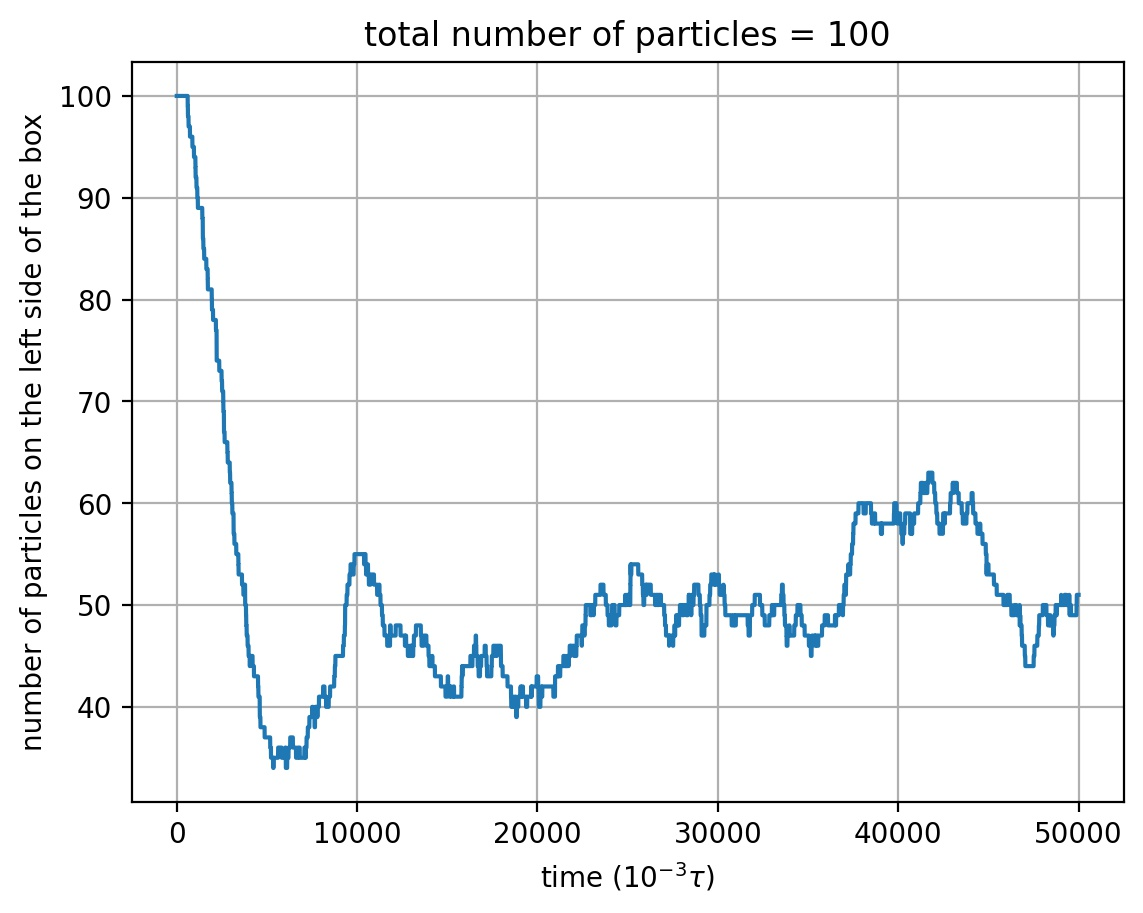
\includegraphics[width=.45\linewidth]{../results/particles_on_left100_50000.jpg}
		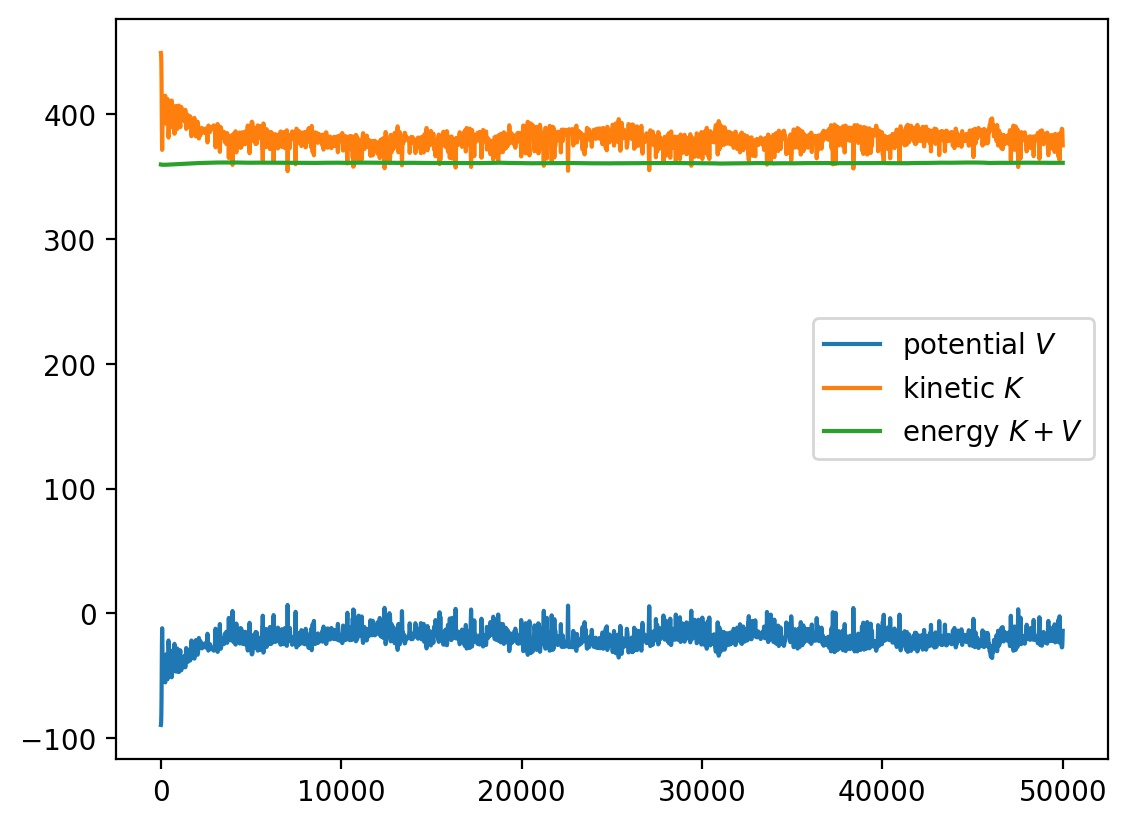
\includegraphics[width=.45\linewidth]{../results/energy_conservation100_50000.jpg}
		\caption{As expected, on the left, we can see that the number of particles on the 
		left side of the box reaches, and oscillates about half of the atoms. And on the right, we
		can clearly witness the conservation of energy}
		\label{fig:energy_and_left}
	\end{figure}

	\subsubsection{Temperature, Pressure, and equilibrium}
	Now, we turn our heads to a thermodynamic observable, temperature. The thermodynamic 
	equation for temperature is:
	\begin{equation}
		\frac{1}{2} \sum_{i=1}^{N}\sum_{e=1}^{d} v_{ie}^2 = Nd \frac{1}{2}k_B T
	\end{equation}
	where $N$ is the number of particles, $d$ is the dimension of the system (in our case 2) and 
	T, the temperature. In the system that $k_B$ is $1$, we can rewrite the equation as follows:
	\begin{equation}
		\sum_{i=1}^{N} \sum_{e=1}^{d} v_{ie}^2 = N d T
	\end{equation}
	one should take note that in our case, we used a convention, namely that the system is 
	stabilized (i.e., the CoM velocity is zero). In Thermodynamics this doesn't matter due to the 
	size of our ensemble, but in MD it matters. So we have:
	\begin{equation*}
		N d T \rightarrow (N-1) d T
	\end{equation*}
	
	Now we use the "Virial Theorem" to find and equation for the pressure of the system.
	\begin{equation}
		P V = N k_B T - \frac{1}{2 N d} \sum_{i,j = 1}^{N} \vec{F}_{ij}.\vec{r}_{ij}
	\end{equation}
	 Now we have an equation to calculate pressure in-time. 
	 
	 The values for temp. and pressure are available in Fig~\ref{fig:temp_pressure}
	 
	 \begin{figure}[h!]
		\centering
		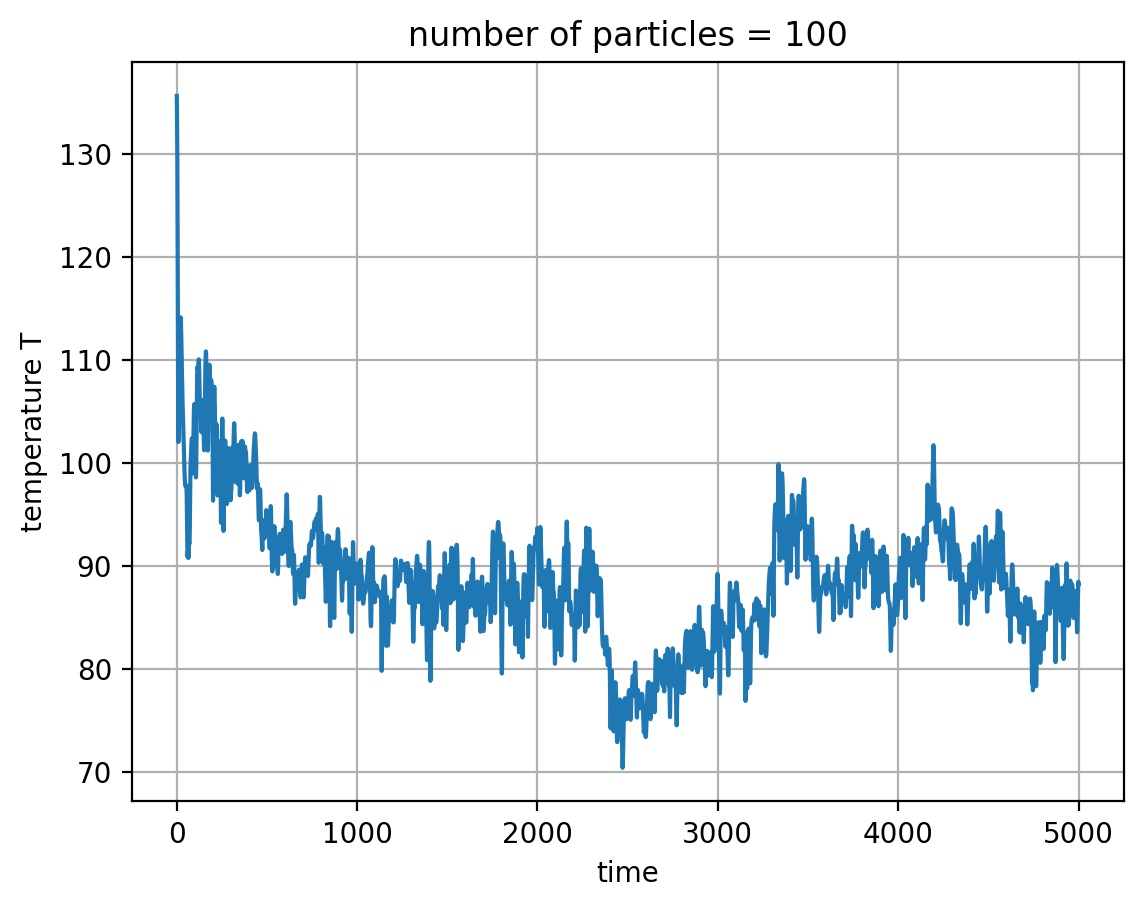
\includegraphics[width=.45\linewidth]{../results/temp100_5000.jpg}
		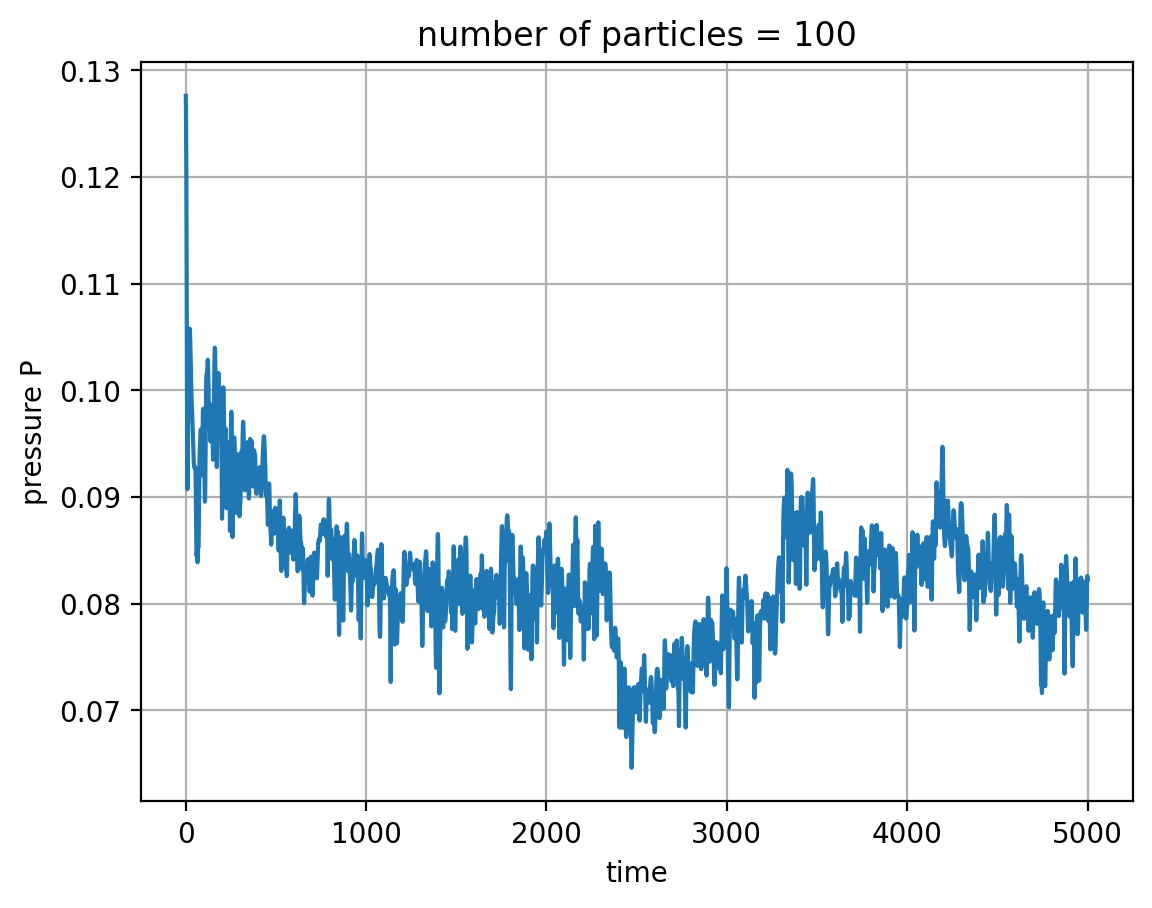
\includegraphics[width=.45\linewidth]{../results/pressure100_5000.jpg}
		\caption{On the left, you can see the plot for temperature over time. the unit for temp. is Kelvin. On the right, you can see the values for 
		reduced pressure. The unit for time on both plots is $10^{-2} \tau$ where $\tau$ is time in reduced units.
		the inital value for velocity is $1.5$}
		\label{fig:temp_pressure}
	 \end{figure}
 
 	We find the temperature and pressure of the system in equilibrium, by taking the mean value over time. The values are found below:
 	\begin{equation*}
 		T_{eq} = 87 \pm 5 K, \; P_{eq} = 0.080 \pm 0.005 \text{(reduced unit)}
 	\end{equation*}
	
	\subsubsection{Velocity Correlation and Relaxation Time}
	I chose the initial conditions to be the same as in the previous section.
	I ran the simulation for 2000 time steps (waiting for the system to reach equilibrium), and then I saved the
	data for the velocity of particles for every 2 time steps in a file in the \texttt{data/} directory.
	
	Then using the file \texttt{velocity\_correlation.py}, I found the correlation and plotted in 
	Fig~\ref{fig:velocity_correlation}
	
	\begin{figure}[h!]
		\centering
		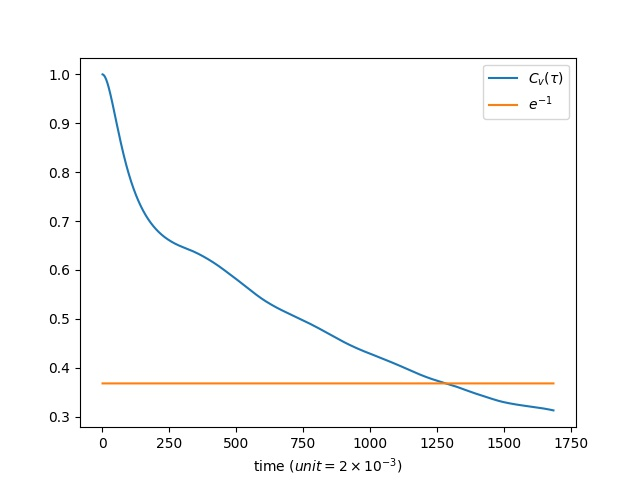
\includegraphics[width=.9\linewidth]{../results/velocity_correlation.jpg}
		\caption{Velocity correlation for different values of seperation $\tau$. The initial velocity in the simulation was 
			$0.5$.}
		\label{fig:velocity_correlation}
	\end{figure}
	
	And so by crossing the auto-correlation curve with the $y = e^{-1}$ line, we find the relation time of the 
	system, $T$, to be:
	\begin{equation}
		T = 2564 \times 10^{-3} \tau = 2.564 \tau, \; \tau \simeq 10^{-12} s \Rightarrow T \simeq 2.564 \times 
		10^{-12} s
	\end{equation}
	
	\subsubsection{State Equation check with the Leonard-Jones gas}
	In order to check this system with the Leonard-Jones gas, I have shown the P-T plot of the system, available in Fig~\ref{fig:P-T}
	\begin{figure}[h!]
		\centering
		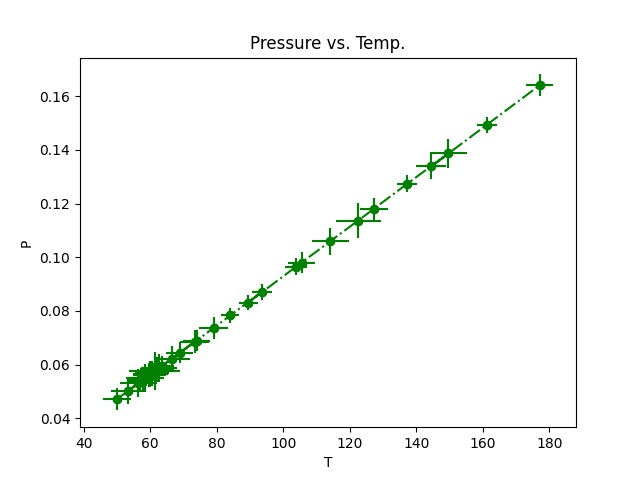
\includegraphics[width=0.9\linewidth]{../results/pressure_temp.jpg}
		\caption{The P-T plot of the system to check with the Leonard-Jones system.}
		\label{fig:P-T}
	\end{figure}
	
	\subsection{Phase transition of the system for different Temperatures}
	In order to see the phase transition of the system we plot the energy E of the system vs. the temperature. And by the change in 
	$C_v = \derivative{E}{T}$ we can see the phase transitions. I varied the energy and temperature of the system by changing the initial velocity
	of the particles. For each initial value, I ran the simulation 2000 time steps for the system to reach equilibrium, then, I ran 5000 times and took
	the temperature of the system and returned the mean and the standard deviation as values and error. The plot is available in 
	Fig~\ref{fig:phase_transition}
	
	\begin{figure}[h!]
		\centering
		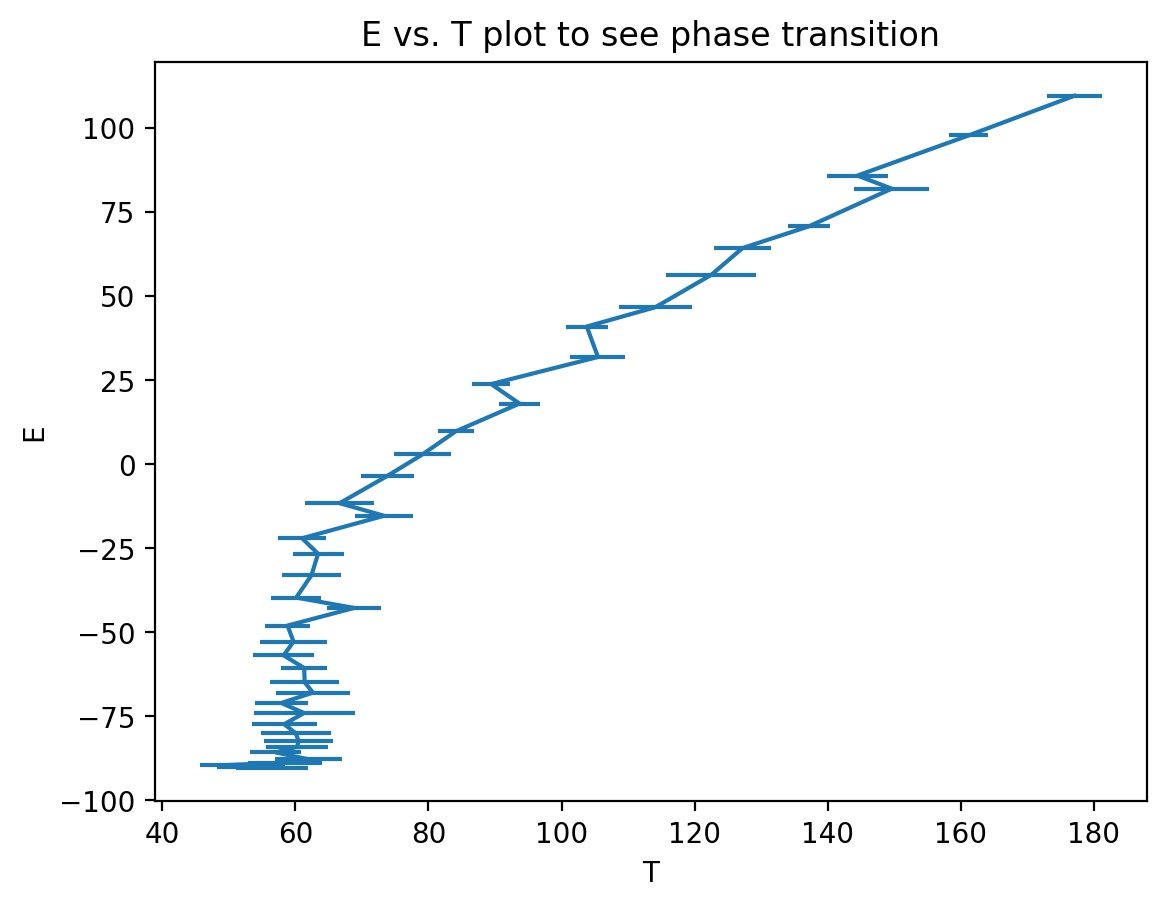
\includegraphics[width=0.9\linewidth]{../results/phase_transition.jpg}
		\caption{Phase Transition of the MD system. As one can see, from about 80 to 90 Kelvin, the system is in the liquid phase, gas for over 90,
		and crystal for lower than 80.}
		\label{fig:phase_transition}
	\end{figure}
	
	\section{Animating the system}
	Again, I wait 2000 time steps for the system to reach equilibrium and then, I start animating the system.
	The initial velocity for the crystal phase is $0.5$, for liquid, $1.5$, and for gas $3$. The animations are accessible in the \texttt{animations/}
	subdirectory.
\end{document}